\documentclass{article}
\usepackage{graphicx}

\usepackage{amsmath}
\usepackage[mathletters]{ucs}
\usepackage[utf8x]{inputenc}
\usepackage{listings}
\lstnewenvironment{code}{\lstset{language=Haskell,basicstyle=\small\ttfamily}}{}
\setlength{\parindent}{0pt}
\setlength{\parskip}{6pt plus 2pt minus 1pt}

\usepackage{array}
% This is needed because raggedright in table elements redefines \\:
\newcommand{\PreserveBackslash}[1]{\let\temp=\\#1\let\\=\temp}
\let\PBS=\PreserveBackslash

\setcounter{secnumdepth}{0}


\begin{document}
\noindent
\begin{tabular}{lr}
CHALMERS TEKNISKA H\"OGSKOLA &Tuesday 16th December, 2009.\\
Dept. of Computer Science and Engineering & Programming Paradigms\\
John Hughes                  & DAT120(CTH) / DIT330(GU) \\
\end{tabular}

\vspace{2.5cm} \noindent
\begin{center} {\LARGE
Exam in Programming Paradigms}
\end{center}

\vspace{1.5cm}

\noindent
Tuesday 16th December, 2007, EM.\\
Lecturer: John Hughes, tel 070 756 3760.
\vspace{1cm}

\noindent
Permitted aids:\\
English-Swedish or English-other language dictionary.

There are five questions, one on each paradigm, worth 12 points each
for a total of 60 points. 24 points is required to pass (grade 3), 36
points is required for grade 4, and 48 points is required for grade 5.

%\newcommand{\comment}[1]{}
\newcommand{\comment}[1]{\marginpar{#1}}

\newpage

\section{Imperative Programming [12 points]}

In this part of the exam, we use the following notation:

\begin{itemize}
\item
  \verb!* q! means: memory cell whose adress is \verb!q!. (Note that
  \verb!q! must be an address)
\item
  \verb!& a! means: address of \verb!a!. (Note that \verb!a! must be
  an l-value)
\end{itemize}

\begin{itemize}
\item Adresses and L-values\hfill{\textbf{[4 points]}}

Which of the following these expressions are l-values? Which expressions are adresses?
(\verb!a!, \verb!b! denote rational
numbers variables; \verb!p!, \verb!q! denote addresses of rational
numbers.)

Reproduce the following table and replace the question marks with
``yes'' or ``no'' appropriately.

\begin{center}
\begin{tabular}{>{\PBS\raggedright\hspace{0pt}}p{0.15\columnwidth}>{\PBS\raggedright\hspace{0pt}}p{0.19\columnwidth}>{\PBS\raggedright\hspace{0pt}}p{0.10\columnwidth}}
expression
 & l-value
 & address
\\
\hline
a
 & ?
 & ?
\\
p
 & ?
 & ?
\\
a + 1
 & ?
 & ?
\\
\& a
 & ?
 & ?
\\
\& p
 & ?
 & ?
\\
* p
 & ?
 & ?
\\
\end{tabular}
\end{center}



\newpage

\item Parameter passing

  
Consider the following program. It uses the ``call by reference''
calling convention.

\begin{verbatim}
f (a, b : integers passed by reference) {    
    a := b
    b := b + 3;
    return t
}

x, y: integer
x := 2;
y := 4;
f(x,y)
x := y + 1;
print (x + y);
\end{verbatim}

What is printed?
\hfill{\textbf{[2 points]}}

Translation to call-by-value. \hfill{\textbf{[6 points]}}

Translate the function \verb!f! \emph{and} its call to a language
that does not support call by reference, but only call by value. Do
so using pointers (use operators \verb!*! and \verb!&!). You are
not allowed to change anything else. In particular, the
``algorithm'' and the declatations of \verb!x! and \verb!y! must
remain the same.

\end{itemize}


\newpage
\section{Object-Oriented Programming [12 points]}

\begin{itemize}

\item Subtyping.

\begin{enumerate}
\item State the substitution principle of Liskov. \hfill{\textbf{[2 points]}}

\item I claim that every type is a subtype of itself. Show that this claim is compatible with 
  the above statement (your answer to the above question) by specialising it. \hfill{\textbf{[2 points]}}
\end{enumerate}

\item Subtyping.

Consider the following axioms to describe semantics of a sort
\verb!S!.

\begin{verbatim}
contains (x, empty) = false
contains (x, insert (x,s)) = true
contains (x, insert (y,s)) = contains (x, s) (assuming x /= y)
remove (x, empty) = empty
remove (x, insert (x,s)) = s
remove (x, insert (y,s)) = insert (y, (remove (x,s)) (assuming x /= y)
insert (x, insert (y,s)) = insert (y, insert (x,s))
\end{verbatim}

\begin{enumerate}
\item 
Write the signature for all operations of the sort \verb!S!. \hfill{\textbf{[3 points]}}

(Assume the sort \verb!Element! for elements, and that Booleans are
pre-defined) 

\item An ADT which implements for this specification must remember the
  number of times that an element is inserted.

Is the previous statement true or false? \hfill{\textbf{[2 points]}}

\item 
By adding an axiom to the above specification, I can change the
answer to the above question. Write down this axiom. \hfill{\textbf{[3 points]}}
\end{enumerate}


\end{itemize}


\newpage

\section{Functional Programming [12 points]}

\begin{enumerate}
\item

Given
\begin{eqnarray*}
\mbox{\it inc}&=&\lambda x.~x+1\\
\mbox{\it twice}&=&\lambda f.~\lambda x.~f~(f~x)
\end{eqnarray*}
use $\beta$-conversion to simplify the following $\lambda$-expression as far as possible:
\[
\mbox{\it twice}~\mbox{\it twice}~\mbox{\it inc}~0
\]
Show each step in your answer.
\comment{1 point}


\item
{\em Church numerals} are a representation of natural numbers as
$\lambda$-expressions, where the $\lambda$-expression $\lambda
f.~\lambda x.~f^n(x)$ represents the natural number $n$. For brevity,
we shall write this $\lambda$-expression as $\hat{n}$. Define
$\lambda$-expressions {\it suc} and {\it add} that implement the
successor and addition functions, such that
\begin{eqnarray*}
\mbox{\it suc}~\hat{n}&=&\widehat{n+1}\\
\mbox{\it add}~\hat{m}~\hat{n}&=&\widehat{m+n}
\end{eqnarray*}
(Note that defining {\em suc} as $\lambda \hat{n}.~\widehat{n+1}$
would make no sense---$\hat{n}$ stands for a $\lambda$-expression, not
a variable name, and indeed, no ``hats'' ($\hat{~}$) should appear in
your answer).
\comment{2 points}


\item
Suppose the Haskell type \verb!Set a! represents a {\em set} of values
of type \verb!a!.
\begin{enumerate}
\item
Suggest suitable types for the functions \verb!insert! and
\verb!delete!, where \verb!insert a s! inserts an element \verb!a!
into the set \verb!s!, and \verb!delete a s! removes an element
\verb!a! from a set \verb!s!.
\comment{1 point}

\item
What will the value of the following expression be, given that
\verb!s! is the set $\{1,2\}$? You may write set values informally
using the usual mathematical notation $\{x_1, x_2, x_3\dots\}$.
\begin{verbatim}
(delete 2 s, insert 3 s)
\end{verbatim}
\comment{1 point}

\end{enumerate}

\item
Sets can be implemented by {\em ordered binary trees}, in which each
node is either a {\em leaf}, or a {\em branch} containing a left
sub-tree, an element, and a right sub-tree, with the invariant that
all the elements in the left sub-tree are less than the element in the
branch node, and all the elements in the right sub-tree are greater
than it. Ordered binary trees can be represented by the following
Haskell type:
\begin{verbatim}
data Set a = Leaf | Branch (Set a) a (Set a)
\end{verbatim}
The following function inserts a new element into such a
tree, in the correct position.
\begin{verbatim}
insert a Leaf = Branch Leaf a Leaf
insert a (Branch l b r) =
  if a==b then Branch l b r
  else if a < b then Branch (insert a l) b r
  else Branch l b (insert a r)
\end{verbatim}
\begin{enumerate}
\item
Given the definition
\begin{verbatim}
t = insert 1 (insert 4 (insert 2 Leaf))
\end{verbatim}
then the following diagram illustrates the value of
\verb!t!.

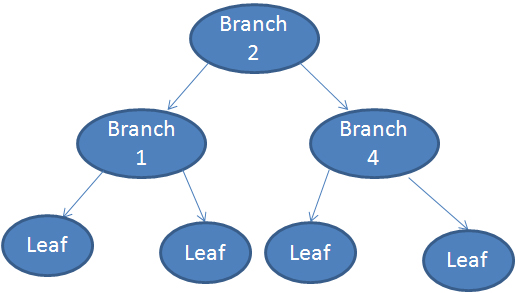
\includegraphics[width=6cm]{tree.jpg} 

Copy this diagram, and {\em in the same diagram} draw the data-structure
returned by \verb!insert 3 t!. Make sure you accurately represent any
sharing between old and new trees.
\comment{1 point}


\item
In your diagram, mark the nodes that will be reclaimed by the garbage
collector assuming that there are no references to \verb!t!, but there
is a reference to the result of \verb!insert 3 t!.
\comment{1 point}


\item
Define a function \verb!delete!, which deletes an element from a tree.
\comment{3 points}


{\em Hint:} you will find you need a function to join together the
left and right subtrees of a branch-node into a single tree. You can
use the following function to do this:
\begin{verbatim}
join Leaf t = t
join (Branch l b r) t = Branch l b (join r t)
\end{verbatim}
There is no need to repeat this definition in your answer.

\item
Suppose the function
\begin{verbatim}
setElements :: Ord a => Set a -> [a]
\end{verbatim}
returns a sorted list of the elements of a set. Write a {\em
  QuickCheck property} that uses an ordered list of elements as a {\em
  model} to test the \verb!insert! function.  You may assume that
QuickCheck can already generate random \verb!Set! values (so you do
not need to define a generator for \verb!Set!s), and you may use the
function \verb!List.insert x xs! that inserts an element \verb!x! into
an ordered list \verb!xs! in the correct position.  \comment{2 points}



\end{enumerate}




\end{enumerate}

\newpage
\section{Concurrency Oriented Programming [12 points]}

Study the following Erlang code, which implements a simple {\em generic server}.
\begin{verbatim}
start_server(M) ->
  register(M,spawn(fun() -> server(M,M:init()) end)).

server(M,S) ->
  receive
    {Pid,Msg} ->
      {Reply,NewS} = M:handle(S,Msg),
      reply(M,Pid,Reply),
      server(M,NewS)
  end.

reply(M,Pid,Msg) ->
  Pid ! {M,Msg}.

rpc(M,Msg) ->
  M ! {self(),Msg},
  receive {M,Reply} -> Reply end.
\end{verbatim}

\begin{enumerate}

\item
What do the following notations mean?
\begin{enumerate}
\item \verb,Pid ! Msg,
\item \verb!receive Msg -> ... end!
\end{enumerate}
\comment{2 points}

\item 
Erlang does not provide locks to protect shared data from simultaneous
modification by two or more concurrent processes. What prevents Erlang
processes from corrupting shared data?
\comment{1 point}

\item
Suppose we want to use the generic server above to create a server
that implements a {\em variable}, with initial value zero, handling
requests \verb!read! to read the variable's value, and
\verb!{write,X}! to set the variable's value to \verb!X!. For example,
we might increment the value held in the variable using the following
code in a client:
\begin{verbatim}
N = rpc(variable,read),
rpc(variable,{write,N+1})
\end{verbatim}
Write definitions of the callback functions \verb!init! and
\verb!handle! to implement this behaviour.
\comment{2 points}

\item
When a client tries to increment the variable's value using the code
above, there is a risk that a different client might change the
variable's value between the read and the write. We might therefore
wish to add two new requests to the server's repertoire: \verb!lock!
  and \verb!unlock!, so that the code above can be written as
\begin{verbatim}
rpc(variable,lock),
N = rpc(variable,read),
rpc(variable,{write,N+1}),
rpc(variable,unlock)
\end{verbatim}
with the effect that the server only accepts requests from this client
between the lock and the unlock. Show how to {\em modify the generic
  server} so that {\em all} servers implemented using it support the
\verb!lock! and \verb!unlock! requests.
\comment{2 points}

{\em Hint:} you can write code such as
\begin{verbatim}
receive 
  {Pid,{write,X}} when X>0 -> 
    ... 
end
\end{verbatim}
to accept a message only when a certain condition holds.

\item
What happens to requests from {\em other} clients, which are sent
while the lock is held?
\comment{1 point}

\item
What is the effect of {\em linking} two Erlang processes?
\comment{1 point}

\item
Show how to modify your generic-server-with-locking, so that if a client
crashes while holding the lock, then
\begin{itemize}
\item the lock is released, so that other clients can use the server,
\item the {\em state} of the server is restored to the value it had
  when the lock was last claimed---so that a client which crashes
  while holding the lock has no visible effect, as far as other
  clients are concerned.
\end{itemize}
\comment{3 points}

\end{enumerate}

\newpage
\section{Logic Programming [12 points]}

\begin{enumerate}
\item
What is the result of unification of the following pairs of terms? In
each case, state whether or not unification succeeds, and if it
succeeds, give the values bound to the variables.  \comment{2 points}

\noindent
\begin{minipage}{0.5\textwidth}
  \begin{enumerate}
  \item
  \verb![X|Xs]! and \verb![1,2,3]!
  \item
  \verb![X,2]! and \verb![1,Y]!
  \item
  \verb![A,A]! and \verb![1,B]!
  \item
  \verb![A,B]! and \verb![1,2,3]!
  \end{enumerate}
\end{minipage}
\begin{minipage}{0.5\textwidth}
  \begin{enumerate}
  \item
  \verb|true| and \verb!X=1! and \verb!Xs=[2,3]!
  \item
  \verb|true| and \verb!X=1! and \verb!Y=2!
  \item
  \verb|true| and \verb!A=B=1!
  \item
  \verb|false|
  \end{enumerate}  
\end{minipage}

\item
Given the clauses
\begin{verbatim}
mem(X,[X|Xs]).
mem(X,[Y|Xs]) :- mem(X,Xs).
\end{verbatim}
what will Prolog display in response to these queries? Make sure to
include all the solutions Prolog will find.
\comment{3 points}

\noindent
\begin{minipage}{0.5\textwidth}
  \begin{enumerate}
  \item \verb!mem(X,[]).!
  \item \verb!mem(X,[1,2,3]).!
  \item \verb!mem(1,X).!
  \end{enumerate}
\end{minipage}
\begin{minipage}{0.5\textwidth}
  \begin{enumerate}
  \item \verb!false!
  \item \verb!true! and (\verb!X=1! or \verb!X=2! or \verb!X=3!)
  \item \verb!true! and \verb!X=[...,1,...]!
  \end{enumerate}
\end{minipage}

\item
Using no more than two clauses, define a predicate \verb!del(X,Xs,Ys)!
which holds when \verb!X! is an element of the list \verb!Xs!, and
removing one \verb!X! from \verb!Xs! leaves the list \verb!Ys!. For
example, given the query \verb!del(2,[1,2,3],Ys)!, Prolog should reply
with \verb!Ys = [1,3]!.
\comment{2 points}

\begin{verbatim}
del(X,[X|Xs],Xs).
del(X,[Y|Xs],[Y|Ys]) :- del(X,Xs,Ys).
\end{verbatim}

\item
What solutions will Prolog find for the queries
\comment{2 points}

\noindent
\begin{minipage}{0.35\textwidth}
  \begin{enumerate}
  \item
  \verb!del(1,[1,2,1],Ys).!
  \item
  \verb!del(3,Xs,[1,2]).!
  \end{enumerate}
\end{minipage}
\begin{minipage}{0.65\textwidth}
  \begin{enumerate}
  \item
  \verb!Ys=[2,1]! or \verb!Ys=[1,2]!
  \item
  \verb!Xs=[3,1,2]! or \verb!Xs=[1,3,2]! or \verb!Xs=[1,2,3]!
  \end{enumerate}
\end{minipage}

\item
Study the following clauses, which define the predicate
\verb!reverse(Xs,Ys)! that holds if the lists \verb!Xs! and
\verb!Ys! are each other's reversal.  
\begin{verbatim}
reverse([],[]).
reverse([X|Xs],Ys) :- reverse(Xs,Zs), append(Zs,[X],Ys).
\end{verbatim}
This uses the \verb!append! predicate from the lectures:
\begin{verbatim}
append([],Ys,Ys).
append([X|Xs],Ys,[X|Zs]) :- append(Xs,Ys,Zs).
\end{verbatim}
\begin{enumerate}
\item
Both of the queries \verb!reverse([1,2,3],Xs)! and
\verb!reverse(Xs,[1,2,3])! find the solution \verb!Xs = [3,2,1]!, but
one of them falls into an infinite loop if we ask for more
solutions. Which query can fall into an infinite loop?
\comment{1 point}

The second (\verb!reverse(Xs,[1,2,3])!) will loop endlessly, because
the code only specifies that \verb!Xs1! should be unified with \verb![X|Xs2]!,
and that \verb!Ys! should be unified with \verb![1,2,3]!. The recursive
use of \verb!reverse! then performs a similar unification, without making
progress.
\item
Using no more than three clauses, give a definition of the
\verb!reverse! predicate which does not fall into a loop in either of
these cases.
\comment{2 points}

\begin{verbatim}
reverse([],[]).
reverse(Xs,[Y|Ys]) :- nonvar(Ys), !, reverse(Ys,Zs), append(Zs,[Y],Xs).
reverse([X|Xs],Ys) :- reverse(Xs,Zs), append(Zs,[X],Ys).
\end{verbatim}

\end{enumerate}

\end{enumerate}

\end{document}
